% WearLens report -- standalone main file (compiles as is on Overleaf with pdfLaTeX).
% When you move to the course template: copy the preamble packages you need, then put
% % ============================================================
% WearLens report -- Sections 2-5 (revision 3, after AI review round 2)
% Title, system name and team members are in main.tex (\title / \author).
% No extra packages required; fallbacks below. Upload figs/motivation.pdf.
% Every number is traceable to the repository (data/verify_expected.json, data/eda_*.csv).
% Naming: end mills are E1-E9 (the dataset calls them T1-T9); tasks are T1-T7.
% ============================================================
\providecommand{\toprule}{\hline}
\providecommand{\midrule}{\hline}
\providecommand{\bottomrule}{\hline}
\providecommand{\url}[1]{\texttt{#1}}

\section{Overview}
During machining, cutting tools wear, and a worn tool degrades product quality and process stability.
Tools are therefore usually replaced after a predefined period, a strategy that wastes much of the
remaining life of most tools~\cite{denkena2023}. Measuring wear directly requires stopping the machine and
inspecting the tool under a microscope. Engineers would therefore like to replace tools based on signals
that the machine control already records. Doing so on several machines is difficult, because tool life and
signal levels differ between machines.
\textbf{WearLens} supports process engineers who introduce tool-condition monitoring on several machine
tools. It helps them compare replacement rules, test whether a production signal can serve as a wear
indicator on a machine it was not calibrated on, and decide whether a suspicious signal change is
caused by wear.

\section{Data and Data Processing}
\paragraph{Source.}
We use the open dataset of Denkena et al.~\cite{denkena2023}
(Mendeley Data, \url{https://doi.org/10.17632/zpxs87bjt8}, CC~BY~4.0). According to its authors, it is the
first public dataset of tool-life trajectories on several machine tools; it has not been used in our course.
Nine solid-carbide end mills of the same model (8\,mm diameter, 4 cutting edges) were each worn from new to
their end of life by shoulder milling of cast iron on three 5-axis machining centres. All machines ran the
same numerical-control (NC) program with identical process parameters. We call the end mills
\textbf{E1--E9} (M1: E1--E3, M2: E4--E6, M3: E7--E9). The M2 end mills come from tool batch B, all others
from batch A. A \emph{run} is one straight milling pass with about 4\,s of cutting, stored as one HDF5 file;
44 runs remove one 2\,mm \emph{layer}, which takes about 2.4\,min of cutting. The dataset has
\textbf{6,418 runs} (10.6\,GB).

\paragraph{Attributes.}
Table~\ref{tab:data} lists the attributes we use. \emph{Flank wear} VB is the width of the worn band on
the flank of the cutting edges, measured under a microscope and averaged over the four edges; the dataset
authors define the end of tool life at $\mathrm{VB}\approx150\,\mu$m. Each run contains time series from
two independent measurement chains: the machine control (500\,Hz) and a dynamometer, a force sensor below
the workpiece (25\,kHz).

\begin{table}[t]
\centering\small
\caption{Attributes used by WearLens (one value per run unless noted).}
\label{tab:data}
\begin{tabular}{@{}p{0.25\linewidth}p{0.21\linewidth}p{0.42\linewidth}@{}}
\toprule
Attribute & Type & Description \\
\midrule
Machine, end mill & categorical & 3 machines, 9 end mills (3 per machine) \\
Run & ordinal & pass counter per end mill (removed runs not counted) \\
Contact time $C$ & quant.\ [s] & cumulated cutting time before the run \\
Flank wear VB & quant.\ [$\mu$m] & microscope measurement, see limitations \\
Layer, pass position & ordinal, quant.\ [mm] & derived from the tool position \\
Machine signals & time series, 500\,Hz & spindle torque; feed-drive \emph{effort}, i.e.\ torque (M1, ball screw) or force (M2/M3, linear motor); position control deviation (commanded minus actual position) \\
Dynamometer forces & time series, 25\,kHz & $F_x, F_y, F_z$; reference only (Section~\ref{sec:users}) \\
\bottomrule
\end{tabular}
\end{table}

\paragraph{Preprocessing (Python, offline).}
After checking all files against their checksums and the dataset's file list, we detect the cutting window of
each run from the dynamometer force (moving root mean square, RMS) and trim 0.15\,s at both ends to exclude
tool entry and exit and a possible 100\,ms misalignment between the two measurement chains. In this window
we compute 21 features: 8 from the machine control (for example the mean absolute spindle torque; absolute
values because the sign convention differs between machines) and 13 from the dynamometer (for example the
force amplitude at the 530\,Hz tooth-passing frequency). We also derive the layer and pass position of each
run and a 200-bin envelope of three signals for drill-down. The browser loads 9.6\,MB of compact files and
computes all analysis components itself. An independent recomputation of two features for 40 random runs
differed by at most $4\times10^{-4}$, and the numbers displayed by the interface match our Python results.

\paragraph{Limitations stated by the dataset authors.}
VB was measured only every one or two layers (about 2.4--4.7\,min of cutting) and is linearly interpolated
in between; we do not identify which values were measured. The first runs of E8 are missing. The spindle
torque and feed-drive force on M2 may be affected by aliasing (distortion because the control's low-pass
filter was disabled). The coordinate system of E7 and E8 was rotated by about 1--2$^\circ$. WearLens shows
these limitations next to the affected views.

\section{Target Users and Analysis Challenges}
\label{sec:users}
\paragraph{Target users.}
Our users are process or maintenance engineers who introduce tool-condition monitoring on several
machine tools. Before deployment they run trials like the one in this dataset: tools are worn on each machine,
machine signals are recorded, and wear is checked with a microscope. A dynamometer may be added in such
a trial, but it is rarely installed in production because it is costly and changes the workpiece clamping.
% TODO: cite a tool-condition-monitoring review that you have checked for this statement.
In production, only the machine-control signals remain, and the microscope is not used during operation.
The trial data are used to decide the rule that will run in production.

\paragraph{Terms and methods.}
A \emph{normalization} makes a feature comparable between end mills. WearLens offers three:
dividing by the same end mill's median in its first 3--6\,min of contact time (computable in production,
because it needs neither the microscope nor future data), dividing by its median at VB\,=\,50--60\,$\mu$m,
and a z-score within each machine (both only possible in a trial). A \emph{signal alarm} fires when the
trailing median of the last 15 runs (about half a layer, computable online) stays above an \emph{alarm level}
for a given number of consecutive runs, the \emph{persistence}. To \emph{calibrate} the level, WearLens takes
the median, over a set of calibration end mills, of their smoothed signal when they reach the VB limit; the set
is either the other two machines, the other end mills of the same machine (leave-one-out), or all end mills of
the machine (in-sample). The \emph{error} of a rule is its replacement or alarm time minus the time at which VB
reaches the limit: negative is \emph{early}, non-negative is \emph{late}; a late replacement is an \emph{overrun},
and an end mill that reaches the limit without an alarm is \emph{missed}. The mean absolute error (MAE) is taken
over the end mills that alarm; missed end mills are always reported separately. The \emph{wear phases} are the fast initial wear, the slow
middle phase and the accelerated final phase visible in Fig.~\ref{fig:motivation}a.
\emph{Spearman's rank correlation} $\rho$ measures how monotonically a feature increases with VB.

\paragraph{CH1: Which replacement rule should be used?}
The engineer can replace tools after a fixed contact time (one time for all machines, or one per machine)
or when a signal alarm fires. Each rule trades unused tool life against the risk of cutting beyond the wear
limit. Tool life varies even under constant parameters~\cite{denkena2023}, and in this dataset it also
differs between machines (Fig.~\ref{fig:motivation}a). This difference cannot be attributed to the
machines alone, because the M2 end mills come from another batch, and each machine has only three end
mills, so any rule fitted to them is optimistic for the next tool. Which rule and which limit to accept is a
judgement that must be made with these uncertainties in view.

\paragraph{CH2: Which production signal can serve as a wear indicator on another machine?}
There are many candidate features and three normalizations. Raw values differ between machines
(Fig.~\ref{fig:motivation}b), and the feed-drive signal even has different units on M1 and M2/M3.
The correlation between a feature and VB within one end mill is inflated, because VB is interpolated from
contact time, so any signal that drifts with time correlates with it. A high correlation is therefore only a
necessary condition; whether an indicator works on a machine it was not calibrated on can only be judged
by testing it there.

\paragraph{CH3: Is a signal change caused by wear?}
Signals also change for reasons other than wear. In Fig.~\ref{fig:motivation}b, the spindle torque of E1
jumps by 19\,\% at the start of layer 15 and falls back in the next layer, although wear cannot decrease.
Machining is interrupted between layers for the microscope measurement, but the dataset does not record
what changed. WearLens flags such layers automatically. A flag, however, only shows \emph{where} a signal
behaves unusually; it does not tell whether an alarm raised in that layer should be trusted, postponed, or
followed by an inspection of the tool. That decision requires looking at the signals around the flagged
layer and at how the alarm depends on it.

\begin{figure}[t]
\centering
\ifdefined\includegraphics
  \IfFileExists{figs/motivation.pdf}{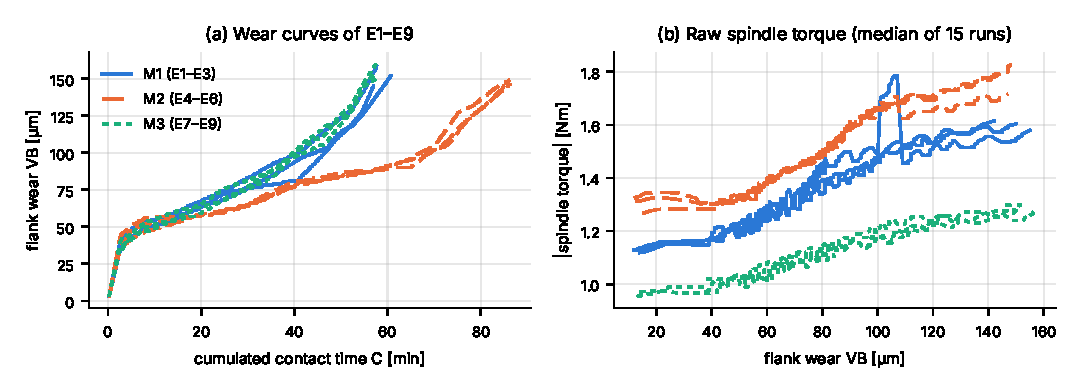
\includegraphics[width=\linewidth]{figs/motivation}}%
    {\fbox{\parbox{0.9\linewidth}{\centering Missing file: upload figs/motivation.pdf}}}
\else
  \fbox{\parbox{0.9\linewidth}{\centering Load graphicx in the preamble to show Fig.~1}}
\fi
\caption{(a) Wear curves of all end mills. (b) Raw spindle torque against wear, smoothed with a median over
15 runs; the levels differ by machine. Colour and line style encode the machine; the three end mills of a
machine are not distinguished here.}
\label{fig:motivation}
\end{figure}

\paragraph{Why visual analytics?}
A single static chart cannot answer these questions: the outcome of a rule depends on the feature,
normalization, calibration, alarm level, persistence and wear limit together. One could search this space
automatically and even mark errors that fall into flagged layers. With three end mills per machine,
however, a single event such as the E1 jump decides whether a setting looks good or bad. Whether that event
should change the rule depends on what it is: a sensor fault, a change in the process, or real wear. Telling
these apart requires comparing the spindle torque, the feed-drive effort and the dynamometer reference
around the event, which is a judgement based on domain knowledge rather than an optimization target.
Choosing between early and missed alarms is, in the end, a decision about cost and quality risk. WearLens therefore
combines the derived measures with the underlying signals so that the engineer can check the measures
before acting on them.

\section{Low-Level Tasks}
Table~\ref{tab:tasks} lists the tasks. T1--T2 address CH1, T3--T4 CH2, and T5--T6 CH3; T7 combines CH1
and CH2 by testing a signal alarm on a machine that was not used for calibration, and T6 links its result back
to CH3. A \emph{time range} is an interval of contact time $C$; a \emph{layer flag} marks a layer whose median
feature value differs from its neighbouring layers (\emph{jump}) or changes within the layer (\emph{rise}) by
more than a user-set percentage. The per-end-mill correlation in T3 is used for screening only (CH2).
The machine--batch confounding cannot be resolved with this data; WearLens labels it wherever machines
are compared, and M1 and M3 (both batch A) can be compared without it.

\begin{table}[t]
\centering\small
\caption{Low-level tasks (end mills are E1--E9; tasks are T1--T7).}
\label{tab:tasks}
\begin{tabular}{@{}p{0.07\linewidth}p{0.66\linewidth}p{0.14\linewidth}@{}}
\toprule
ID & Task (task type) & From \\
\midrule
T1 & Overview the wear curves of all end mills and compare in which wear phase the machines differ \emph{(overview, compare)} & CH1 \\
T2 & For a chosen VB limit, compare the unused life and the overrun of fixed-time rules \emph{(compare, derive)} & CH1 \\
T3 & Screen features by Spearman $\rho$ with VB, per end mill and pooled, and compare the ranking between normalizations and time ranges \emph{(rank, correlate)} & CH2 \\
T4 & Compare the normalized trend of one feature across the three machines \emph{(compare)} & CH2 \\
T5 & Identify layers whose jump or rise exceeds a user-set percentage \emph{(detect outliers)} & CH3 \\
T6 & For an early alarm, check whether it was raised in a flagged layer, compare the signals of that layer with the previous one and with the dynamometer reference, and decide whether to trust the alarm \emph{(verify, details on demand)} & CH3, CH1 \\
T7 & Calibrate an alarm level on two machines, test it on the third, and compare the alarm error for different persistence settings \emph{(derive, compare)} & CH1, CH2 \\
\bottomrule
\end{tabular}
\end{table}
 after \begin{document} and \maketitle.
\documentclass[10pt,twocolumn]{article}
\usepackage[utf8]{inputenc}
\usepackage[T1]{fontenc}
\usepackage[margin=2cm]{geometry}
\usepackage{booktabs}
\usepackage{graphicx}
\usepackage{hyperref}

\title{WearLens: Visual Analytics of End-Mill Wear across Machine Tools}
\author{Name A (Student ID, email) \and Name B (Student ID, email) \and Name C (Student ID, email)} % TODO
\date{}

\begin{document}
\maketitle
% ============================================================
% WearLens report -- Sections 2-5 (revision 3, after AI review round 2)
% Title, system name and team members are in main.tex (\title / \author).
% No extra packages required; fallbacks below. Upload figs/motivation.pdf.
% Every number is traceable to the repository (data/verify_expected.json, data/eda_*.csv).
% Naming: end mills are E1-E9 (the dataset calls them T1-T9); tasks are T1-T7.
% ============================================================
\providecommand{\toprule}{\hline}
\providecommand{\midrule}{\hline}
\providecommand{\bottomrule}{\hline}
\providecommand{\url}[1]{\texttt{#1}}

\section{Overview}
During machining, cutting tools wear, and a worn tool degrades product quality and process stability.
Tools are therefore usually replaced after a predefined period, a strategy that wastes much of the
remaining life of most tools~\cite{denkena2023}. Measuring wear directly requires stopping the machine and
inspecting the tool under a microscope. Engineers would therefore like to replace tools based on signals
that the machine control already records. Doing so on several machines is difficult, because tool life and
signal levels differ between machines.
\textbf{WearLens} supports process engineers who introduce tool-condition monitoring on several machine
tools. It helps them compare replacement rules, test whether a production signal can serve as a wear
indicator on a machine it was not calibrated on, and decide whether a suspicious signal change is
caused by wear.

\section{Data and Data Processing}
\paragraph{Source.}
We use the open dataset of Denkena et al.~\cite{denkena2023}
(Mendeley Data, \url{https://doi.org/10.17632/zpxs87bjt8}, CC~BY~4.0). According to its authors, it is the
first public dataset of tool-life trajectories on several machine tools; it has not been used in our course.
Nine solid-carbide end mills of the same model (8\,mm diameter, 4 cutting edges) were each worn from new to
their end of life by shoulder milling of cast iron on three 5-axis machining centres. All machines ran the
same numerical-control (NC) program with identical process parameters. We call the end mills
\textbf{E1--E9} (M1: E1--E3, M2: E4--E6, M3: E7--E9). The M2 end mills come from tool batch B, all others
from batch A. A \emph{run} is one straight milling pass with about 4\,s of cutting, stored as one HDF5 file;
44 runs remove one 2\,mm \emph{layer}, which takes about 2.4\,min of cutting. The dataset has
\textbf{6,418 runs} (10.6\,GB).

\paragraph{Attributes.}
Table~\ref{tab:data} lists the attributes we use. \emph{Flank wear} VB is the width of the worn band on
the flank of the cutting edges, measured under a microscope and averaged over the four edges; the dataset
authors define the end of tool life at $\mathrm{VB}\approx150\,\mu$m. Each run contains time series from
two independent measurement chains: the machine control (500\,Hz) and a dynamometer, a force sensor below
the workpiece (25\,kHz).

\begin{table}[t]
\centering\small
\caption{Attributes used by WearLens (one value per run unless noted).}
\label{tab:data}
\begin{tabular}{@{}p{0.25\linewidth}p{0.21\linewidth}p{0.42\linewidth}@{}}
\toprule
Attribute & Type & Description \\
\midrule
Machine, end mill & categorical & 3 machines, 9 end mills (3 per machine) \\
Run & ordinal & pass counter per end mill (removed runs not counted) \\
Contact time $C$ & quant.\ [s] & cumulated cutting time before the run \\
Flank wear VB & quant.\ [$\mu$m] & microscope measurement, see limitations \\
Layer, pass position & ordinal, quant.\ [mm] & derived from the tool position \\
Machine signals & time series, 500\,Hz & spindle torque; feed-drive \emph{effort}, i.e.\ torque (M1, ball screw) or force (M2/M3, linear motor); position control deviation (commanded minus actual position) \\
Dynamometer forces & time series, 25\,kHz & $F_x, F_y, F_z$; reference only (Section~\ref{sec:users}) \\
\bottomrule
\end{tabular}
\end{table}

\paragraph{Preprocessing (Python, offline).}
After checking all files against their checksums and the dataset's file list, we detect the cutting window of
each run from the dynamometer force (moving root mean square, RMS) and trim 0.15\,s at both ends to exclude
tool entry and exit and a possible 100\,ms misalignment between the two measurement chains. In this window
we compute 21 features: 8 from the machine control (for example the mean absolute spindle torque; absolute
values because the sign convention differs between machines) and 13 from the dynamometer (for example the
force amplitude at the 530\,Hz tooth-passing frequency). We also derive the layer and pass position of each
run and a 200-bin envelope of three signals for drill-down. The browser loads 9.6\,MB of compact files and
computes all analysis components itself. An independent recomputation of two features for 40 random runs
differed by at most $4\times10^{-4}$, and the numbers displayed by the interface match our Python results.

\paragraph{Limitations stated by the dataset authors.}
VB was measured only every one or two layers (about 2.4--4.7\,min of cutting) and is linearly interpolated
in between; we do not identify which values were measured. The first runs of E8 are missing. The spindle
torque and feed-drive force on M2 may be affected by aliasing (distortion because the control's low-pass
filter was disabled). The coordinate system of E7 and E8 was rotated by about 1--2$^\circ$. WearLens shows
these limitations next to the affected views.

\section{Target Users and Analysis Challenges}
\label{sec:users}
\paragraph{Target users.}
Our users are process or maintenance engineers who introduce tool-condition monitoring on several
machine tools. Before deployment they run trials like the one in this dataset: tools are worn on each machine,
machine signals are recorded, and wear is checked with a microscope. A dynamometer may be added in such
a trial, but it is rarely installed in production because it is costly and changes the workpiece clamping.
% TODO: cite a tool-condition-monitoring review that you have checked for this statement.
In production, only the machine-control signals remain, and the microscope is not used during operation.
The trial data are used to decide the rule that will run in production.

\paragraph{Terms and methods.}
A \emph{normalization} makes a feature comparable between end mills. WearLens offers three:
dividing by the same end mill's median in its first 3--6\,min of contact time (computable in production,
because it needs neither the microscope nor future data), dividing by its median at VB\,=\,50--60\,$\mu$m,
and a z-score within each machine (both only possible in a trial). A \emph{signal alarm} fires when the
trailing median of the last 15 runs (about half a layer, computable online) stays above an \emph{alarm level}
for a given number of consecutive runs, the \emph{persistence}. To \emph{calibrate} the level, WearLens takes
the median, over a set of calibration end mills, of their smoothed signal when they reach the VB limit; the set
is either the other two machines, the other end mills of the same machine (leave-one-out), or all end mills of
the machine (in-sample). The \emph{error} of a rule is its replacement or alarm time minus the time at which VB
reaches the limit: negative is \emph{early}, non-negative is \emph{late}; a late replacement is an \emph{overrun},
and an end mill that reaches the limit without an alarm is \emph{missed}. The mean absolute error (MAE) is taken
over the end mills that alarm; missed end mills are always reported separately. The \emph{wear phases} are the fast initial wear, the slow
middle phase and the accelerated final phase visible in Fig.~\ref{fig:motivation}a.
\emph{Spearman's rank correlation} $\rho$ measures how monotonically a feature increases with VB.

\paragraph{CH1: Which replacement rule should be used?}
The engineer can replace tools after a fixed contact time (one time for all machines, or one per machine)
or when a signal alarm fires. Each rule trades unused tool life against the risk of cutting beyond the wear
limit. Tool life varies even under constant parameters~\cite{denkena2023}, and in this dataset it also
differs between machines (Fig.~\ref{fig:motivation}a). This difference cannot be attributed to the
machines alone, because the M2 end mills come from another batch, and each machine has only three end
mills, so any rule fitted to them is optimistic for the next tool. Which rule and which limit to accept is a
judgement that must be made with these uncertainties in view.

\paragraph{CH2: Which production signal can serve as a wear indicator on another machine?}
There are many candidate features and three normalizations. Raw values differ between machines
(Fig.~\ref{fig:motivation}b), and the feed-drive signal even has different units on M1 and M2/M3.
The correlation between a feature and VB within one end mill is inflated, because VB is interpolated from
contact time, so any signal that drifts with time correlates with it. A high correlation is therefore only a
necessary condition; whether an indicator works on a machine it was not calibrated on can only be judged
by testing it there.

\paragraph{CH3: Is a signal change caused by wear?}
Signals also change for reasons other than wear. In Fig.~\ref{fig:motivation}b, the spindle torque of E1
jumps by 19\,\% at the start of layer 15 and falls back in the next layer, although wear cannot decrease.
Machining is interrupted between layers for the microscope measurement, but the dataset does not record
what changed. WearLens flags such layers automatically. A flag, however, only shows \emph{where} a signal
behaves unusually; it does not tell whether an alarm raised in that layer should be trusted, postponed, or
followed by an inspection of the tool. That decision requires looking at the signals around the flagged
layer and at how the alarm depends on it.

\begin{figure}[t]
\centering
\ifdefined\includegraphics
  \IfFileExists{figs/motivation.pdf}{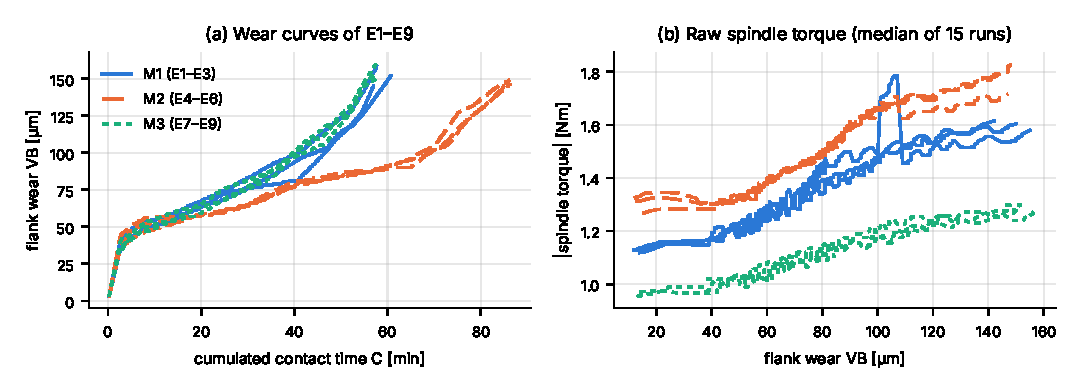
\includegraphics[width=\linewidth]{figs/motivation}}%
    {\fbox{\parbox{0.9\linewidth}{\centering Missing file: upload figs/motivation.pdf}}}
\else
  \fbox{\parbox{0.9\linewidth}{\centering Load graphicx in the preamble to show Fig.~1}}
\fi
\caption{(a) Wear curves of all end mills. (b) Raw spindle torque against wear, smoothed with a median over
15 runs; the levels differ by machine. Colour and line style encode the machine; the three end mills of a
machine are not distinguished here.}
\label{fig:motivation}
\end{figure}

\paragraph{Why visual analytics?}
A single static chart cannot answer these questions: the outcome of a rule depends on the feature,
normalization, calibration, alarm level, persistence and wear limit together. One could search this space
automatically and even mark errors that fall into flagged layers. With three end mills per machine,
however, a single event such as the E1 jump decides whether a setting looks good or bad. Whether that event
should change the rule depends on what it is: a sensor fault, a change in the process, or real wear. Telling
these apart requires comparing the spindle torque, the feed-drive effort and the dynamometer reference
around the event, which is a judgement based on domain knowledge rather than an optimization target.
Choosing between early and missed alarms is, in the end, a decision about cost and quality risk. WearLens therefore
combines the derived measures with the underlying signals so that the engineer can check the measures
before acting on them.

\section{Low-Level Tasks}
Table~\ref{tab:tasks} lists the tasks. T1--T2 address CH1, T3--T4 CH2, and T5--T6 CH3; T7 combines CH1
and CH2 by testing a signal alarm on a machine that was not used for calibration, and T6 links its result back
to CH3. A \emph{time range} is an interval of contact time $C$; a \emph{layer flag} marks a layer whose median
feature value differs from its neighbouring layers (\emph{jump}) or changes within the layer (\emph{rise}) by
more than a user-set percentage. The per-end-mill correlation in T3 is used for screening only (CH2).
The machine--batch confounding cannot be resolved with this data; WearLens labels it wherever machines
are compared, and M1 and M3 (both batch A) can be compared without it.

\begin{table}[t]
\centering\small
\caption{Low-level tasks (end mills are E1--E9; tasks are T1--T7).}
\label{tab:tasks}
\begin{tabular}{@{}p{0.07\linewidth}p{0.66\linewidth}p{0.14\linewidth}@{}}
\toprule
ID & Task (task type) & From \\
\midrule
T1 & Overview the wear curves of all end mills and compare in which wear phase the machines differ \emph{(overview, compare)} & CH1 \\
T2 & For a chosen VB limit, compare the unused life and the overrun of fixed-time rules \emph{(compare, derive)} & CH1 \\
T3 & Screen features by Spearman $\rho$ with VB, per end mill and pooled, and compare the ranking between normalizations and time ranges \emph{(rank, correlate)} & CH2 \\
T4 & Compare the normalized trend of one feature across the three machines \emph{(compare)} & CH2 \\
T5 & Identify layers whose jump or rise exceeds a user-set percentage \emph{(detect outliers)} & CH3 \\
T6 & For an early alarm, check whether it was raised in a flagged layer, compare the signals of that layer with the previous one and with the dynamometer reference, and decide whether to trust the alarm \emph{(verify, details on demand)} & CH3, CH1 \\
T7 & Calibrate an alarm level on two machines, test it on the third, and compare the alarm error for different persistence settings \emph{(derive, compare)} & CH1, CH2 \\
\bottomrule
\end{tabular}
\end{table}


\bibliographystyle{plain}
\bibliography{refs}
\end{document}
